\chapter{Adresy a smerníky (pointre)}

Technicky je celá pamäť počítača jedno veľké pole núl a jednotiek. V skutočnosti má
adresu iba každý ôsmy bit (celá pamäť teda vyzerá ako pole \prg!unsigned char!).
Keby na adrese 1 bola premenná \prg!int c;!, na adrese 5
premenná \prg!char a! a na adrese 6 premenná \prg!char b;!
začiatok pamäte by mohol vyzerať takto:


\centerline{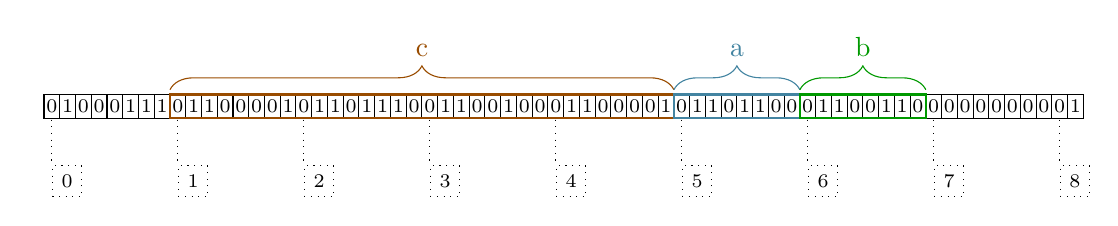
\begin{tikzpicture}[scale=0.2]
  \def\var#1[#2]#3#4{%
    \pgfmathsetmacro{\tmp}{#1+8*#2}
    \draw[#4] decorate[
       decoration={brace, amplitude=2ex}]{
       (#1,1.8) -- (\tmp,1.8) node [align=center,midway,anchor=south,yshift=2ex] {\vb{#3}}
        };
   \draw[#4,thick] (#1,0) rectangle (\tmp,1.5);

  }
  \foreach \v [count=\i] in {
    0,1,0,0,0,1,1,1,
    0,1,1,0,0,0,0,1,
    0,1,1,0,1,1,1,0,
    0,1,1,0,0,1,0,0,
    0,1,1,0,0,0,0,1,
    0,1,1,0,1,1,0,0,
    0,1,1,0,0,1,1,0,
    0,0,0,0,0,0,0,0,
    0,1
  }{
    \draw (\i,0) rectangle node [anchor=center] {{\scriptsize\roboto \v}} (\i+1,1.5);
  }

  \foreach \i in {0,...,8}{
    \pgfmathsetmacro{\x}{\i*8+1.5}
  \draw[dotted] (\x,-0.1) -- (\x,-3) 
  node[draw, anchor = north west]{\scriptsize\vb{\i}};
}

  \var{9}[4]c{orange!60!black}
  \var{41}[1]a{cyan!60!black}
  \var{49}[1]b{green!60!black}
\end{tikzpicture}}


To, že nejaká premenná je na nejakej adrese, nie je v pamäti nijak špeciálne označené, je 
na programe, aby pristupoval na správne miesta v pamäti. V pamäti je vždy okrem tvojho 
programu veľa ďalších vecí, takže keď sa program spustí, operačný systém nájde v pamäti
voľné miesto a tvoj program bude používať adresy odtiaľ. Presná adresa premennej ti preto
sama osebe veľa nepovie, napriek tomu je užitočné ju vedieť. Až tak užitočné, že na to je
špeciálny operátor, \indexItem{Prg}{operátor \vb{\&}}\vb{\&}. Ak máš premennú \vb{x}, tak \vb{\&x} je jej adresa.
Skús si spustiť program:\\


\vbox{
\begin{lstlisting}[] 
#include <iostream>
using namespace std;

int c;
char a,b;

int main() {
  cout <<"adresa c: "<< (unsigned long)&c << endl;
  cout <<"adresa a: "<< (unsigned long)&a << endl;
  cout <<"adresa b: "<< (unsigned long)&b << endl;
} 
\end{lstlisting}
}

Vždy, keď ho spustíš, vypíšu sa iné čísla (tvoj program vždy dostane pridelenú
inú časť pamäte), ale môže to vyzerať napr. takto:

\begin{outputBox}
adresa c: 94082916049300
adresa a: 94082916049304
adresa b: 94082916049305
\end{outputBox}

V tomto prípade sa premenná \vb{c} uložila na adresu $94082916049300$ a zaberá 4 byty
(32 bitov). Za ňou, na adrese $94082916049304$ nasleduje premenná \vb{a}, ktorá zaberá
jeden byte, takže na nasledujúcej adrese $94082916049305$ je premenná \vb{b}.

\indexItem{Prg}{typ pointer}
Napriek tomu, že adresa je vždy číslo, operátor \prg!&! vracia v skutočnosti rôzne
typy. Pre každý typ \vb{T} (základný alebo vlastný
napr. \prg!int!, \prg!float!, \prg!Farba!,\ldots) existuje ďalší typ 
\cmd{adresa premennej typu \vb{T}} (hovorí sa aj {\em pointer na premennú typu \vb{T}}).
Tento nový typ sa označuje hviezdičkou za menom typu. Takže premenná typu \prg!int*! 
obsahuje adresu premennej, ktorá
je typu \prg!int!:\\



\vbox{
\begin{lstlisting}[] 
#include <iostream>
using namespace std;
int main() {
  int x = 258;       // premenná
  int *ax = &x;      // ok, ax je adresa x
  float *err = &x;   // <--  !! error: cannot convert 'int*' to 'float*'
  float* fx = (float*)(&x);  // ok, pretypovať sa dá
}
\end{lstlisting}
}

V poslednom riadku som použil pretypovanie; \vb{fx} je adresa miesta, kde by mala byť
premenná typu \prg!float!, aj keď v skutočnosti je tam uložená premenná typu \prg!int! 
(konkrétne \vb{x}). Ešte raz treba zdôrazniť: premenná \vb{ax} je krabička, v ktorej
je uložené číslo adresy\footnote{%
  V nasledujúcom obrázku ťa zámerne trochu klamem, v premennej typu \vb{int} sa väčšinou
  jej 4 byty ukladajú v opačnom poradí (tzv. {\em little endian}), ale pre
  naše účely to stačí takto.
}, na ktorej je uložená krabička s menom \vb{x}:

\centerline{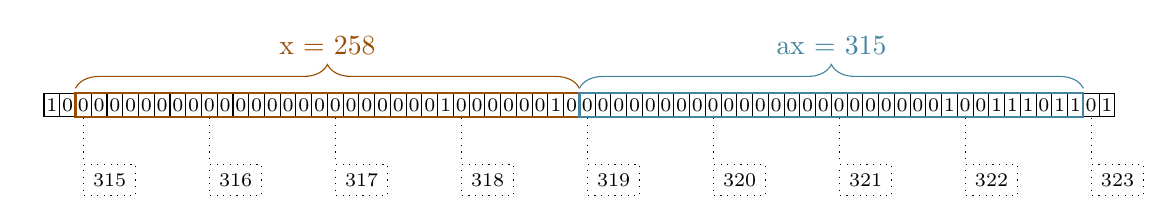
\begin{tikzpicture}[scale=0.2]
  \def\var#1[#2]#3#4{%
    \pgfmathsetmacro{\tmp}{2+#1+8*#2}
    \draw[#4] decorate[
       decoration={brace, amplitude=2ex}]{
       (2+#1,1.8) -- (\tmp,1.8) node [align=center,midway,anchor=south,yshift=2ex] {\vb{#3}}
        };
   \draw[#4,thick] (2+#1,0) rectangle (\tmp,1.5);

  }
  \foreach \v [count=\i] in {
    1,0,
    0,0,0,0,0,0,0,0,
    0,0,0,0,0,0,0,0,
    0,0,0,0,0,0,0,1,
    0,0,0,0,0,0,1,0,
    %
    0,0,0,0,0,0,0,0,
    0,0,0,0,0,0,0,0,
    0,0,0,0,0,0,0,1,
    0,0,1,1,1,0,1,1,
    0,1
  }{
    \draw (\i,0) rectangle node [anchor=center] {{\scriptsize\roboto \v}} (\i+1,1.5);
  }

  \foreach \i in {0,...,8}{
    \pgfmathsetmacro{\x}{\i*8+3.5}
    \pgfmathtruncatemacro{\l}{\i+315}
  \draw[dotted] (\x,-0.1) -- (\x,-3) 
  node[draw, anchor = north west]{\scriptsize\vb{\l}};
}

  \var{1}[4]{x = 258}{orange!60!black}
  \var{33}[4]{ax = 315}{cyan!60!black}
\end{tikzpicture}}


\indexItem{Prg}{operátor \vb{*}} Opačný operátor k \prg!&! je \prg!*!: ak \prg!ax! je premenná typu \prg!int*!, tak
\prg!*ax! je premenná, ktorá je uložená na adrese, ktorá je uložená v  \vb{ax}
(hovoríme, že premenná \vb{ax} {\em ukazuje na premennú} \vb{*ax}). 
Teraz je vidno, prečo je
dobré mať zvlášť typ adresy pre každý typ: keď sa vyhodnocuje výraz \prg!*ax!, procesor
sa pozrie do premennej \vb{ax}, nájde tam číslo (napr. 315), pozrie sa na adresu $315$
a predpokladá, že tam bude premenná typu \prg!int!. Pozrie sa preto na nasledujúce
4 byty a vráti príslušné číslo. V predchádzajúcom príklade by \prg!cout << *ax << endl;! vypísalo $258$.
\prg!*ax! je naozaj premenná, takže sa dá do nej aj priraďovať. Príkazy
\prg!x = 47;! a \prg!(*ax) = 47;! urobia to isté. Takže program\\


\vbox{
\begin{lstlisting}[] 
#include <iostream>
using namespace std;
int main() {
  int x = 258;       
  int* ax = &x;  // ax ukazuje na x   
  (*ax) = 47;    // *ax je x
  cout << x << endl;
}
\end{lstlisting}
}
vypíše 47.


Treba rozlišovať medzi hviezdičkou pri vyrábaní premennej (napr. \prg!int *a!), ktorá znamená
\cmd{pointer na typ int} a hviezdičkou pred menom premennej (typu pointer) vo výraze,
ktorá znamená \cmd{hodnota na adrese}. Skús prečítať nasledovný program:\\


\vbox{
\begin{lstlisting}[] 
#include <iostream>
using namespace std;

int main() {
  int a = 7, x = 6;  // a,x sú premenné typu int
  int *b = &a;       // b ukazuje na a
  int **c = &b;      // c ukazuje na b
  int *d = *c;       // *c je premenná b, preto tento príkaz
                     // je rovnaký ako int* d = b;
  **c = 18;
  b = &x;            // teraz b ukazuje na x
  **c = 42;          
  cout << a << " " << x << endl;
}
\end{lstlisting}
}

Po prvých štyroch riadkoch by to v pamäti mohlo vyzerať ako na obrázku vľavo.
V príkaze \prg!**c=18;! je \prg!*c! premenná \prg!b! a \prg!*b! je premenná \prg!a!,
preto sa do premennej \prg!a! zapíše 18.
Nasledujúci príkaz \prg!b=&x! spôsobí, že v \vb{b} bude uložená adresa \vb{x} ako na 
obrázku vpravo. Preto v príkaze \prg!**c=42! je \prg!*c! premenná \prg!b!
a \prg!*b! je premenná \prg!x!, takže program vypíše \vb{18 42}.


\def\var(#1)#2#3#4{%
  \draw (0,0.5-#1)  node[anchor=east]{\vb{#3}};
  \draw (0.2,-#1) rectangle node[align=center]{\vb{#2}} (1.2,1-#1);
  \draw (1.4,0.5-#1) node[anchor=west]{\textcolor{magenta}{\vb{#4}}};
}

\def\ptr(#1,#2)[#3] {
  \draw[blue,-{>[length=4pt,width=2.5pt]}] (1.7,0.5-#1) to[out=#3,in=-#3] (1.7,0.5-#2);
}

\begin{column}{0.45}
\begin{tikzpicture}[yscale=0.4,xscale=1.4]
  \node[anchor=east] at (0,0.8){{\em adresa}};
  \foreach \val/\addr/\name[count=\i] in {7/42380/a,6/42384/x,42380/42388/b,
     42388/42396/c,42380/42404/d}  {
    \var(\i){\val}{\addr}{\name}
  }
  \draw(0,0.5-6) node[anchor=east]{\vb{42412}};
  \draw[draw=none] (0.2,-6) rectangle node[align=center]{\vb{\ldots}} (1.2,1-6);
  \ptr(3,1)[75]
  \ptr(4,3)[60]
  \ptr(5,1)[65]
\end{tikzpicture}
\end{column}
\hfill
\begin{column}{0.45}
\begin{tikzpicture}[yscale=0.4,xscale=1.4]
  \node[anchor=east] at (0,0.8){{\em adresa}};
  \foreach \val/\addr/\name[count=\i] in {18/42380/a,6/42384/x,42384/42388/b,
     42388/42396/c,42380/42404/d}  {
    \var(\i){\val}{\addr}{\name}
  }
  \draw(0,0.5-6) node[anchor=east]{\vb{42412}};
  \draw[draw=none] (0.2,-6) rectangle node[align=center]{\vb{\ldots}} (1.2,1-6);
  \ptr(3,2)[60]
  \ptr(4,3)[60]
  \ptr(5,1)[65]
\end{tikzpicture}
\end{column}


S pomocou pointrov môžeš mať funkciu, ktorá ako keby menila svoje parametre.
Porovnaj tieto dva programy:


\begin{column}{0.45}
\vbox{
\begin{lstlisting}[] 
#include <iostream>
using namespace std;

void pridaj(int a) { 
  a = a + 1; 
}

int main() {
  int x = 7;
  pridaj(x);
  cout << x << endl;
} 
\end{lstlisting}
}
\end{column}
\hfill
\begin{column}{0.45}
\vbox{
\begin{lstlisting}[] 
#include <iostream>
using namespace std;

void pridaj(int *a) {
  (*a) = (*a) + 1;
}

int main() {
  int x = 7;
  pridaj(&x);
  cout << x << endl;
}
\end{lstlisting}
}
\end{column}

V ľavom programe sa vyrobí svet funkcie \vb{main} a v ňom premenná \vb{x}. Pri
volaní funkcie \vb{pridaj} sa vyrobí nový svet s premennou \vb{a} a nastaví sa jej
hodnota na $7$. Potom sa vykoná funkcia \vb{pridaj}, takže v premennej \vb{a}
bude $8$. Svet funkcie \vb{pridaj} potom zanikne a v \vb{main} sa vypíše hodnota 
\vb{x}, t.j. 7. V pravom programe sa vyrobí svet funckie \vb{pridaj}, ale 
premenná \vb{a} sa nastaví na adresu premennej \vb{x} (premenná \vb{x} je vo svete 
funkcie \vb{main}, ale svety a premenné sú vec programu a kompilátora; pri prístupe
do pamäte vo výslednej binárke nehrajú rolu).
Preto vo svete \vb{pridaj}  výraz \vb{*a} označuje premennú \vb{x} zo sveta funkcie \vb{main}
a funkcia \vb{pridaj} zvýši hodnotu \vb{x} o 1. Keď svet \vb{pridaj}
zanikne, zanikne premenná \vb{a}, ale hodnota \vb{x} ostane zmenená.


\def\var(#1)#2#3#4{%
  \draw (0,0.5-#1)  node[anchor=east]{\vb{#3}};
  \draw (0.2,-#1) rectangle node[align=center]{\vb{#2}} (1.2,1-#1);
  \draw (1.4,0.5-#1) node[anchor=west]{\textcolor{magenta}{\vb{#4}}};
}

\def\ptr(#1,#2)[#3] {
  \draw[blue,-{>[length=4pt,width=2.5pt]}] (1.7,0.5-#1) to[out=#3,in=-#3] (1.7,0.5-#2);
}

\def\kon(#1)#2{ \draw(0,0.5-#1) node[anchor=east]{\vb{#2}};
  \draw[draw=none] (0.2,-#1) rectangle node[align=center]{\vb{\ldots}} (1.2,1-#1);
}

\def\world(#1)#2#3{
  \draw[thick,#3](-1,-#1) -- (2,-#1) node[anchor=west]{\vb{#2}};
}
\begin{column}{0.45}
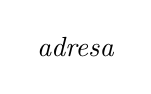
\begin{tikzpicture}[yscale=0.4,xscale=1.4]
  \node[anchor=east] at (0,0.8){{\em adresa}};
  \world(0){main}{orange}
  \world(1){pridaj}{blue!70!gray}

  \foreach \val/\addr/\name[count=\i] in {7/873200/x,8/873204/a}  {
    \var(\i){\val}{\addr}{\name}
  }
  
  \kon(3){873208}
\end{tikzpicture}
\end{column}
\hfill
\begin{column}{0.45}
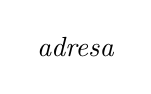
\begin{tikzpicture}[yscale=0.4,xscale=1.4]
  \node[anchor=east] at (0,0.8){{\em adresa}};
  \world(0){main}{orange}
  \world(1){pridaj}{blue!70!gray}

  \foreach \val/\addr/\name[count=\i] in {8/873200/x,837200/873204/a}  {
    \var(\i){\val}{\addr}{\name}
  }
  \ptr(2,1)[70]
  \kon(3){873208}
\end{tikzpicture}
\end{column}

\indexItem{Prg}{pointrová aritmetika}
S pointrami sa dajú robiť aj aritmetické operácie, ale trochu inak ako s normálnymi
číslami. Ak k premennej typu pointer pripočítaš 1, zväčší sa o veľkosť typu, na ktorý
ukazuje (v prípade \prg!int! je to 4). Veľkosť typu sa dá zistiť pomocou príkazu
\prg!sizeof!. V poli sú prvky uložené za sebou, takže napr. program

\vbox{
\begin{lstlisting}[] 
#include <iostream>
using namespace std;

int main() {
  int a = {12, 35};  // a[0] a a[1] nasledujú v pamäti za sebou
  int *x = &(a[0]);
  cout << *x << " " << *(x + 1) << endl;
  cout << (unsigned long)x << " + " << sizeof(int) << " = "
       << (unsigned long)(x + 1) << endl;
}
\end{lstlisting}
}

mi vypísal

\begin{outputBox}
12 35
140727139715200 + 4 = 140727139715204
\end{outputBox}

Pri práci s pointrami si treba dávať pozor na to, aby vždy ukazovali do pamäte,
ktorá patrí tvojmu programu. Môžeš napríklad napísať \prg!int *a = (int*)856;!
a nič zlé sa nestane. Ale ak by si potom chcel urobiť \prg!*a = 3;!, program skončí
s hláškou \vb{Segmentation fault}: pamäť na adrese 856 ti nepatrí. Je dobrý zvyk
do pointrov, ktoré zatiaľ neukazujú na nič rozumné, priradiť 0 (adresa 0 ti celkom
isto nepatrí) a pred použitím urobiť test. Môžeš napísať \prg!int *a = 0;!, alebo
\prg!int *a = NULL;! alebo \prg!int *a = nullptr;!, všetky tri spravia v konečnom 
dôsledku to isté.


\indexItem{Prg}{pointer na pole a pole pointrov}
Samozrejme, pointer môže ukazovať aj na vlastné typy a dokonca aj na polia.
To môže byť trochu zamotané. Napr.\\

\vbox{
\begin{lstlisting}[] 
int a, b, c;
int *p[3] = {&a, &b, &c};

*(p[0]) = 5;
*(p[1]) = 25;
*(p[2]) = 225;

cout << a << " " << b << " " << c << endl;
\end{lstlisting}
}

vyrobí trojprvkové pole \vb{p}, ktorého prvky budú pointre na premenné typu \prg!int!
a naplní ho pointrami na premenné \vb{a, b, c}. Preto potom \prg!p[0]! je pointer
na premennú \prg!a! a teda \prg!*(p[0]) = 5;! priradí 5 do premennej \vb{a}
a program vypíše \vb{5 25 225}. Zápis \prg!int *p[3]! čítaš najprv od 
názvu premennej doprava
a potom doľava zvyšok: \cmd{pole dĺžky 3, ktorého prvky sú pointre na int}.
Ak napíšeš \prg!int (*p)[3]!, znemená to \cmd{pointer na pole dĺžky 3,
ktorého prvky sú int}:\\

\vbox{
\begin{lstlisting}[] 
int a[3] = {1, 2, 3};
int(*p)[3] = &a;

cout << (*p)[1] << endl;
\end{lstlisting}
}

Ako by si zapísal pole dĺžky 2, ktorého prvky sú polia dĺžky 3? \prg!int a[2][3]!
Pripomína ti to niečo? Presne tak, je to dvojrozmerné pole. Dvojrozmerné pole
je vlastne pole riadkov, ktorého prvky sú polia stĺpcov. Preto môžeš mať\\

\vbox{
\begin{lstlisting}[] 
int a[2][3] = {{1, 2, 3}, {4, 5, 6}};
int(*p)[3] = &(a[0]);

cout << (*(p+1))[1] << endl;
\end{lstlisting}
}

V tomto prípade \vb{a} je pole dĺžky 2, ktorého prvky sú trojprvkové polia,
preto \vb{a[0]} je trojprvkové pole.
\vb{p} je pointer na trojprvkové pole, preto môžeš napísať \prg!p=&(a[0])!.
Potom \prg!p+1! ukazuje do pamäte o 12 bytov ďalej (\prg!sizeof(int[3])! je 12).
Prvky v poli sú uložené za sebou, preto 
ak \prg!p! ukazuje na \prg!a[0]!, tak \prg!p+1! ukazuje na \prg!a[1]!.
Napokon \prg!*(p+1)! je to isté, čo \prg!a[1]!, preto \prg!(*(p+1))[1]! vypíše 5.

